\section{Uvod}

\subsection{Commodore 1541}
\textit{Commodore 1541} je čitač \textit{5.25"} flopi disketa korićenih u radu sa \textit{Commodore 64} računarima. Razvijen je u Kanadi od strane kompanije Commodore, 1982. godine \cite{Commodore1541Text}. Izgled ovog čitača prikazan je na slici \ref{img:commodore1541}.
\begin{figure}[ht]
\begin{center}
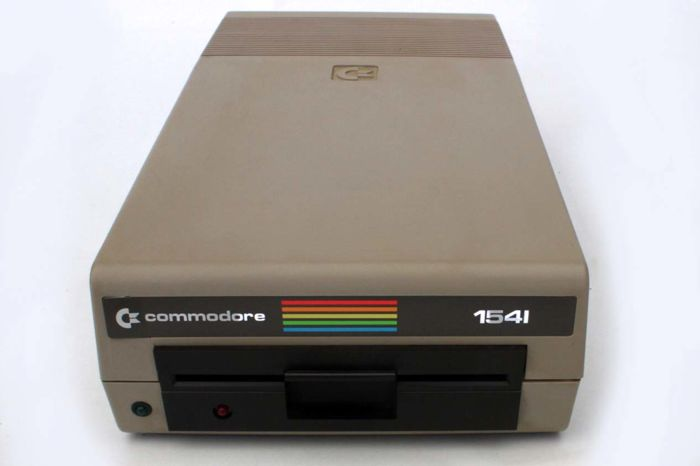
\includegraphics[width=11cm]{img/Commodore1541.jpg}
\caption[Commodore 1541 \textit{(preuzeto \cite{Commodore1541})}]{Commodore 1541}
\label{img:commodore1541}
\end{center}
\end{figure}

Originalna \textit{5.25"} flopi disketa imala je 35 kružnih traka na kojima su bili raspoređeni sektori od po 256 bajta. Postojala je i verzija sa 40 traka. Trake su imale različit broj sektora i bile su raspoređene od spolja ka unutra, odnosno prva traka je bila bliža spoljašnjoj ivici i imala je najviše sektora, dok je 35 traka bila bliža unutrašnjem prstenu diskete sa najmanje sektora \cite{D64}. Broj sektora po trakama je prikazan u tabeli \ref{tab:sektor_traka}.
\begin{table}[h!]
\begin{center}
\begin{tabular}{ | c | c| c | c | } 
\hline
Traka & Sektori/traka & Ukupno Sektora & Skladište u bajtima \\
\hline
\hline
1-17 & 21 & 357 & 7820 \\
\hline
18-24 & 19 & 133 & 7170 \\
\hline
25-30 & 18 & 108 & 6300 \\
\hline
31-35(40) & 17 & 85 & 6020 \\
\hline
\end{tabular}
\end{center}
\caption{Broj sektora po traci \textit{5.25"} flopi diskete}
\label{tab:sektor_traka}
\end{table}

\subsection{D64 fajl}
\textit{D64 fajl} je elektronska byte predstava \textit{5.25"} flopi diskete \textit{Commodore 64} računara. Standardni \textit{D64 file} ima 174848 bajtova, 683 sektora sa po 256 bajta i on oslikava originalnu \textit{5.25"} flopi disketu sa 35 traka.  Postoji i verzija ovog fajla sa 196608 bajtova,768 sektora sa po 256 bajta koja oslikava verziju \textit{5.25"} flopi diskete sa 40 traka \cite{D64}.

Na kraju \textit{D64 fajla} mogu se naći error bajtovi, koji govore koji sektori imaju problem. Ukoliko se na kraju fajla ne pojave error bajtovi to znači da su svi sektori ispravni. Veličina fajlova u zavisnosti od error bajtova je prikazana u tabeli \ref{tab:error_velicina}.
\begin{table}[h!]
\begin{center}
\begin{tabular}{ | c | c |} 
\hline
Tip diskete & Veličina(bajt) \\
\hline
\hline
35 traka, no errors & 174848 \\
\hline
35 traka, 689 error bajtova & 175531 \\
\hline
40 traka, no errors & 196608 \\
\hline
40 traka, 768 error bajtova & 197376 \\
\hline
\end{tabular}
\end{center}
\caption{Veličina fajla u zavisnosti od error bajtova}
\label{tab:error_velicina}
\end{table}
